\section{Course Introduction}

The concepts and techniques in this course are probably the most useful in engineering. A {\it signal} is a function of one or more independent variables conveying information about a physical (or virtual) phenomena. A {\it system} may respond to signals to produce other signals, or produce signals directly.

\begin{center}
  \begin{tikzpicture}[auto, node distance=3cm,>=latex']
    \node [input, name=input] {};
    \node [block, right of=input] (system) {System $T$};
    \node [output, right of=system] (output) {};

    \draw [draw,->] (input) -- node {Input $x$} (system);
    \draw [->] (system) -- node {Output $y$} (output);
  \end{tikzpicture}
\end{center}

This course is about the mathematical models and related techniques for the design and understanding of systems as signal transformations. We focus on a broadly useful class of systems, known as {\it linear, time-invariant systems}. You will learn about:

\begin{itemize}
\item the representation and analysis of signals as information carrying channels
\item and how to analyze and implement linear, time-invariant systems to transform those signals.
\end{itemize}

\begin{example} Electrical Circuits. This is a Sallen-Key filter, a second-order system commonly use to select frequencies from a signal:
  \begin{center}
    \begin{circuitikz}[american voltages,scale=0.8, every node/.style={transform shape}]
      \draw
      (7,3.5) node[op amp] (opamp1) {}
      (0,4) to[R,l=$R_1$,o-] (2,4)
      (2,4) to[short] (2,5)
      (2,5) to[C,l=$C_1$] (8.2,5)
      (8.2,5) to[short] (opamp1.out) 
      (2,4) to[R, l=$R_2$] (4,4)
      (4,4) to[C, l=$C_2$] (4,0)
      (0,0) to[short,o-o] (12,0)
      (4,4) to[short] (opamp1.-)
      (opamp1.+) to[short] (5.8,1.75)
      (5.8,1.75) to[short] (8.2,1.75)
      (opamp1.out) to[R, l=$(1-\beta)R$] (8.2,1.75)
      (8.2,1.75) to[R, l=$\beta R$] (8.2,0)
      (opamp1.out) to[short, -o] (12,3.5)
      (0,4) to[open, v=$x(t)$] (0,0)
      (12,3.5) to[open, v=$y(t)$] (12,0);
    \end{circuitikz}
  \end{center}
  How do we choose the values of the resistors and capacitors to select the frequencies we are interested in? How do we determine what those frequencies are?
\end{example}

\begin{example} Robotic Joint. This is a Linear, Time-Invariant model of a DC motor, a mixture of electrical and mechanical components.

  \begin{center}
    \tikzstyle{block} = [draw, fill=gray!20, rectangle, 
      minimum height=3em, minimum width=3em]
    \tikzstyle{sum} = [draw, fill=gray!20, circle, node distance=1cm]
    \tikzstyle{input} = [coordinate]
    \tikzstyle{output} = [coordinate]
    \tikzstyle{pinstyle} = [pin edge={to-,thin,black}]

    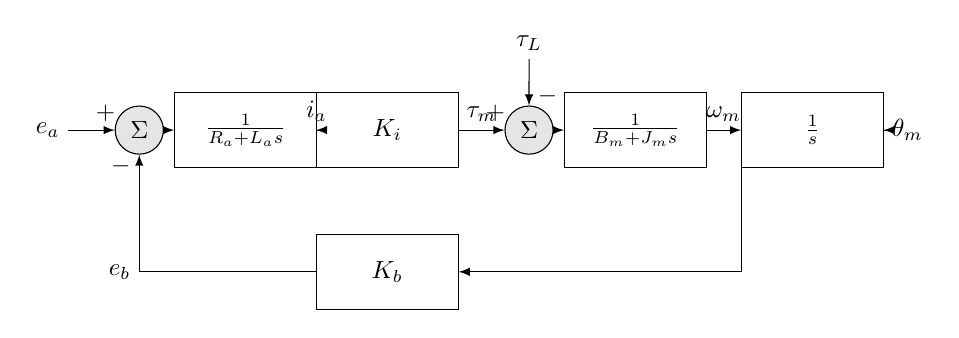
\begin{tikzpicture}[auto, node distance=2cm,>=latex, scale=0.9, every node/.style={transform shape}]

      \node [sum] at (2.5,0) (vsum) {$\Sigma$};
      \node [block] at (4,0) (arm) {$\frac{1}{R_a + L_a s}$};
      \node [block] at (6,0) (torque) {$K_i$};
      \node [sum] at (8,0) (tsum) {$\Sigma$};
      \node [block] at (9.5,0) (motor) {$\frac{1}{B_m + J_m s}$};
      \node [block] at (12,0) (int) {$\frac{1}{s}$};
      \node [block] at (6,-2) (backemf) {$K_b$};

      \draw [->] (1.5,0) node [left] {$e_a$} -- node[pos=0.8] {$+$} (vsum);
      \draw [->] (vsum) -- (arm);
      \draw [->] (arm) -- (torque) node [midway,above] {$i_a$};
      \draw [->] (torque) -- node[pos=0.8] {$+$} (tsum) node [midway,above] {$\tau_m$};
      \draw [->] (tsum) -- (motor);
      \draw [->] (8,1) node[above] {$\tau_L$} -- node[pos=0.8] {$-$} (tsum);
      \draw [->] (motor) -- (int) node [midway,above] {$\omega_m$};
      \draw [->] (11,0) |- (backemf);
      \draw [->] (backemf) -| node[midway] {$e_b$} node[pos=0.95] {$-$} (vsum);
      \draw [->] (int) -- (13,0) node[right] {$\theta_m$};
    \end{tikzpicture}
  \end{center}
  
  How do we convert the motor into a servo for use in a robotic joint? What are its characteristics (e.g. how fast can it move)?
\end{example}

\begin{example} Audio Processing. Suppose you record an interview for a podcast, but during an important part of the discussion, the HVAC turns on and there is an annoying noise in the background.

  \begin{center}
    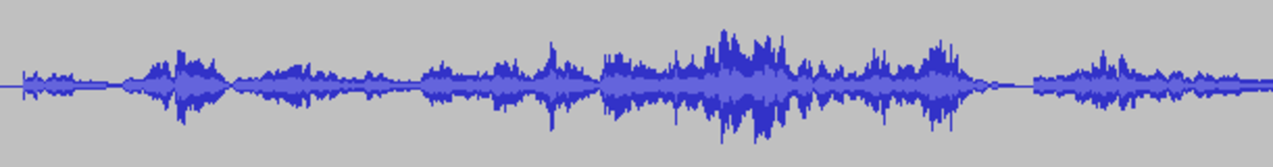
\includegraphics[scale=0.5]{figures/noisysignal.pdf}
  \end{center}

  How could you remove the noise minimizing distortion to the rest of the audio?
\end{example}

\begin{example} Communications. Consider a wireless sensor, that needs to transmit to a base station, e.g. a wireless mic system. 
  \begin{center}
    \tikzset{block/.style = {draw, fill=white, rectangle,
        minimum height=3em, minimum width=2cm},
      input/.style = {coordinate},
      output/.style = {coordinate},
      pinstyle/.style = {pin edge={to-,t,black}},
      radiation/.style={decorate,decoration={expanding waves,angle=12,segment length=4pt}}
    }
    \begin{tikzpicture}[auto, node distance=2cm,>=latex']
      \node[block](tx){Sensor Node};
      \node[antenna] at (tx.east) {};
      \node[block,right = 5cm of tx](rx){Base Station};
      \node[antenna,xscale=-1] at (rx.west) {};

      \draw[radiation] ([shift={(1cm,2cm)}]tx.east)-- node [above=5mm] {} ([shift={(-1cm,2cm)}]rx.west);
    \end{tikzpicture}
  \end{center}

  How should the signal be processed so it can be transmitted? How should the received signal be processed?
\end{example}

\subsection*{Types of Problems}
Applications of this material occur in all areas of science and engineering. When we have a measured output but are unsure what combination of inputs and system components could have produced it, we have a {\it modeling} problem.

\begin{center}
  \begin{tikzpicture}[auto, node distance=3cm,>=latex']
    \node [input, name=input] {};
    \node [block, right of=input] (system) {?};
    \node [output, right of=system] (output) {};

    \draw [draw,->] (input) -- node {Input ?} (system);
    \draw [->] (system) -- node {Output $y$} (output);
  \end{tikzpicture}
\end{center}

Models are the bedrock of the scientific method and are required to apply the concepts of this course to engineering problems. 

When we know the input and the system description and desire to know the output we have an {\it analysis} problem. 

\begin{center}
  \begin{tikzpicture}[auto, node distance=3cm,>=latex']
    \node [input, name=input] {};
    \node [block, right of=input] (system) {System $T$};
    \node [output, right of=system] (output) {};

    \draw [draw,->] (input) -- node {Input $x$} (system);
    \draw [->] (system) -- node {Output ?} (output);
  \end{tikzpicture}
\end{center}

Analysis problems are the kind you have encountered most often already. For example, given an electrical circuit and an applied voltage or current, what are the voltages and currents across and through the various components.

When we know either the input and desired output and seek the system to perform this transformation,
\begin{center}
  \begin{tikzpicture}[auto, node distance=3cm,>=latex']
    \node [input, name=input] {};
    \node [block, right of=input] (system) {System ?};
    \node [output, right of=system] (output) {};

    \draw [draw,->] (input) -- node {Input $x$} (system);
    \draw [->] (system) -- node {Output $y$} (output);
  \end{tikzpicture}
\end{center}

or we know the system description and output and desire the input that would generate the output,

\begin{center}
  \begin{tikzpicture}[auto, node distance=3cm,>=latex']
    \node [input, name=input] {};
    \node [block, right of=input] (system) {System $T$};
    \node [output, right of=system] (output) {};

    \draw [draw,->] (input) -- node {Input ?} (system);
    \draw [->] (system) -- node {Output $y$} (output);
  \end{tikzpicture}
\end{center}

we have a {\it design problem}.

This course focuses on modeling and analysis with applications to electrical circuits and devices for measurement and control of the physical world and is broadly applicable to all ECE majors. Some Examples:

\begin{itemize}
\item Controls, Robotics, \& Autonomy: LTI systems theory forms the basis of perception and control of machines.
\item Communications \& Networking: LTI systems theory forms the basis of transmission and reception of signals, e.g. AM and FM radio.
\item Machine Learning: LTI systems are often used to pre-process samples or to create basis functions to improve learning.
\item Energy \& Power Electronic Systems: linear circuits are often modeled as LTI systems.
\end{itemize}

Subsequent courses, e.g. ECE 3704, focus more on analysis and design.

\subsection*{Learning Objectives}

The learning objectives (LOs) for the course are:
\begin{enumerate}
\item[LO-1] Describe a given system using a block-level description and identify the input/output signals.
\item[LO-2] Mathematically model continuous and discrete linear, time-invariant systems using differential and difference equations respectively.
\item[LO-3] Analyze the use of filters and their interpretation in the time and frequency domains and implement standard filters in hardware and/or software.
\item[LO-4] Apply computations of the four fundamental Fourier transforms to the analysis and design of linear systems.
\item[LO-5] Communicate solutions to problems and document projects within the domain of signals and systems through formal written documents.
\end{enumerate}

These are broken down further into the following topic learning objectives (TLOs). These are well covered in the course Textbook "Oppenheim, A. V., Willsky, A. S., and Nawab, S. H. Signals and Systems. ii, Essex UK: Prentice Hall Pearson, 1996." (abbreviated OW). This is an older, but very good book. However there are many, many texts that cover the same material. \textit{Engaged} reading the textbook is one of the most important things you can do to learn this material. Importantly, these notes should \textbf{not} be considered a replacement for the textbook.

\begin{enumerate}
\item[TLO-1] Course introduction (OW Forward and \S 1.0)
  \begin{enumerate}
  \item Signals as models
  \item Systems as transformation of signals
  \item Prerequisites
  \end{enumerate}

\item[TLO-2] Continuous-time (CT) signals (OW \S 1.1 through 1.4 and 2.5)
  \begin{enumerate}
  \item Continuous-time signals as functions $\mathbb{R}\mapsto\mathbb{C}$
  \item Transformations of time
  \item Characterizing signals
    \begin{enumerate}
    \item periodic/aperiodic
    \item even/odd
    \item energy or/nor power
    \end{enumerate}
  \item Impulse function
  \item Step function
  \item Complex exponential
  \end{enumerate}

\item[TLO-3] Discrete-time (DT) signals (OW \S 1.1 through 1.4)
  \begin{enumerate}
  \item Discrete-time signals as functions $\mathbb{Z}\mapsto\mathbb{C}$
  \item Transformations of time index
  \item Characterizing signals
    \begin{enumerate}
    \item periodic/aperiodic
    \item even/odd
    \item energy or/nor power
    \end{enumerate}
  \item Impulse function
  \item Step function
  \item Complex exponential
  \end{enumerate}

\item[TLO-4] CT systems as linear constant coefficient differential equations (OW \S 2.4.1)
  \begin{enumerate}
  \item LCCDE and their solution (1st and 2nd order)
  \item impulse response from LCCDE
  \end{enumerate}
  
\item[TLO-4] DT systems as linear constant coefficient difference equations (OW \S 2.4.2)
  \begin{enumerate}
  \item LCCDE and their solution (1st and 2nd order)
  \item impulse response from LCCDE
  \end{enumerate}
  
\item[TLO-5] Linear time invariant CT systems (OW \S 1.5, 1.6, 2.3)
  \begin{enumerate}
  \item Memory
  \item Invertability
  \item Causality
  \item Stability
  \item Time-invariance
  \item Linearity
  \item Define LTI system
  \end{enumerate}

\item[TLO-6] Linear time invariant DT systems (OW \S 1.5, 1.6, 2.3)
  \begin{enumerate}
  \item Memory
  \item Invertability
  \item Causality
  \item Stability
  \item Time-invariance
  \item Linearity
  \item Define LTI system
  \end{enumerate}

\item[TLO-7] CT convolution (OW \S 2.2)
  \begin{enumerate}
  \item Review CT LTI systems and superposition property
  \item CT Convolution Integral
  \item Properties of convolution
    \begin{enumerate}
    \item communative 
    \item distributive
    \item associative
    \end{enumerate}
  \item Determining system response using convolution with impulse response
  \end{enumerate}

\item[TLO-8] DT convolution (OW \S 2.1)
  \begin{enumerate}
  \item Review DT LTI systems and superposition property
  \item DT Convolution Sum
  \item Properties of convolution
    \begin{enumerate}
    \item communative 
    \item distributive
    \item associative
    \end{enumerate}
  \item Determining system response using convolution with impulse response
  \end{enumerate}
  
\item[TLO-9] CT block diagrams (OW \S 1.5.2 and 2.4.3)
  \begin{enumerate}
  \item blocks represented by impulse response
  \item series and parallel connections, reductions
  \item scale, sum, and integrator blocks
  \item equivalence of LCCDE's and block diagrams
  \item first-order differential equation as feedback motif
  \item second-order differential equation as a feedback motif
  \item implementing a LCCDE using adders, multipliers, and integrators
  \end{enumerate}

\item[TLO-10] DT block diagrams (OW \S 1.5.2 and 2.4.3)
  \begin{enumerate}
  \item blocks represented by impulse response
  \item series and parallel connections, reductions
  \item scale, sum, and unit delay blocks
  \item equivalence of LCCDE's and block diagrams
  \item first-order difference equation as feedback motif
  \item second-order difference equation as a feedback motif
  \item implementing a LCCDE using adders, multipliers, and delays
  \end{enumerate}

\item[TLO-11] Eigenfunctions of CT systems (OW \S 3.2 and 3.8)
  \begin{enumerate}
  \item Eigenfunction $e^{st}$
  \item Transfer Function $H(s)$
  \item Stability and Frequency Response (FR)  $H(j\omega)$
  \item How this is useful - decomposition of input signal into complex exp
  \item What signals can be decomposed this way, foreshadow Fourier Analysis
  \end{enumerate}
  
\item[TLO-12] Eigenfunctions of DT systems (OW \S 3.2 and 3.8)
  \begin{enumerate}
  \item Eigenfunction $z^{n}$
  \item Transfer Function $H(z)$
  \item Stability and Frequency Response (FR) $H\left(e^{j\omega}\right)$
  \item How this is useful - decomposition of input signal into complex exp
  \item What signals can be decomposed this way, foreshadow Fourier Analysis
  \end{enumerate}
  
\item[TLO-13] CT Fourier Series representation of signals (OW \S 3.3 through 3.5)
  \begin{enumerate}
  \item review CT periodic functions
  \item harmonic sums
  \item derive synthesis equation
  \item derive analysis equation
  \item spectrum plots
  \item define mean-square convergence
  \item truncated CT FS
  \item stable LTI system response using CTFS
  \item example of the impulse train (for sampling theory later)
  \item formal Dirichlet conditions
  \item properties of CT FS
  \end{enumerate}

\item[TLO-14] DT Fourier Series representation of signals  (OW \S 3.6 and 3.7)
  \begin{enumerate}
  \item review DT periodic functions
  \item harmonic sums
  \item derive synthesis equation
  \item derive analysis equation
  \item spectrum plots
  \item stable LTI system response using DTFS
  \item properties of DT FS
  \end{enumerate}
  
\item[TLO-15] CT Fourier Transform (OW \S 4.0 through 4.7)
  \begin{enumerate}
  \item derive the CTFT pair from the CTFS 
  \item Dirichlet existence conditions
  \item CTFT of the CTFS
  \item Properties of the CT Fourier Transform
    \begin{enumerate}
    \item linearity
    \item time shift
    \item conjugacy
    \item integration and differentiation: application to LCCDE $\mapsto$ CTFR
    \item time scaling
    \item duality
    \item convolution: stable LTI system response using CTFT
    \item multiplication/modulation
    \item application of the properties in combination
    \end{enumerate}
  \end{enumerate}

\item[TLO-16] DT Fourier Transform (OW \S 5.0 though 5.8)
  \begin{enumerate}
  \item derive the DTFT from DTFS
  \item DTFT of DTFS
  \item Properties of the DT Fourier Transform
    \begin{enumerate}
    \item periodicity
    \item linearity
    \item index-shift: application to LCCDE $\mapsto$ DTFR
    \item frequency shift
    \item conjugation
    \item finite difference and accumulation
    \item interpolation /index expansion
    \item frequency differentiation
    \item Parseval's
    \item convolution: stable LTI system response using DTFT
    \item multiplication/modulation
    \item application of the properties in combination
    \end{enumerate}
  \end{enumerate}

\item[TLO-17] CT Frequency Response (OW \S 6.1, 6.2, 6.5)
  \begin{enumerate}
  \item review CTFR as CTFT of impulse response
  \item review CTFR to/from LCCDE
  \item review CTFR to/from block diagram 
  \item magnitude-phase representation of the frequency response
  \item frequency response acting on sinusoids
  \item Bode plots
    \begin{enumerate}
    \item why plot it this way: dB units and log time axis
    \item how to read them (\textbf{not} construct them manually)
    \item Bode plots in software, e.g. Matlab/Python/Julia
    \end{enumerate}
  \item CTFR of first and second order systems
  \end{enumerate}

\item[TLO-18] DT Frequency Response (OW \S 6.1, 6.2, 6.6)
  \begin{enumerate}
  \item review DTFR as DTFT of impulse response
  \item review DTFR to/from LCCDE
  \item review DTFR to/from block diagram 
  \item magnitude-phase representation of the frequency response
  \item frequency response acting on sinusoids
  \item DTFR plots  
    \begin{enumerate}
    \item periodicity
    \item dB units
    \item DTFR plots in software, e.g. Matlab/Python/Julia
    \end{enumerate}
  \item DTFR of first and second order systems
  \end{enumerate}
  
\item[TLO-19] Frequency Selective Filters in CT (OW \S 3.9, 3.10, 6.3, 6.4) 
  \begin{enumerate}
  \item ideal low-pass
  \item ideal high-pass
  \item ideal bandpass
  \item ideal notch/bandstop
  \item practical filters
  \item transformations
  \item first and second order systems as building blocks
    \begin{enumerate}
    \item review LCCDE representation
    \item review block diagram representation
    \item review CTFR representation
    \item CT 1st order RC+buffer
    \item CT Sallen-key
    \end{enumerate}
  \end{enumerate}
  
\item[TLO-20] Frequency Selective Filters in DT (OW \S 3.11, 6.3, 6.4)
  \begin{enumerate}
  \item ideal low-pass
  \item ideal high-pass
  \item ideal bandpass
  \item ideal notch/bandstop
  \item practical filters
  \item transformations
  \item first and second order systems as building blocks
    \begin{enumerate}
    \item review LCCDE representation
    \item review block diagram representation
    \item review DTFR representation
    \item DT 1st order implementation in code
    \item DT 2nd order implementation in code
    \end{enumerate}
  \end{enumerate}
  
\item[TLO-21] The Discrete Fourier Transform
  \begin{enumerate}
  \item time window the DTFT to get the DFT
  \item interpreting the index axis as DT and CT frequency
  \item zero-padding
  \item offline or batched filtering using the DFT
  \item briefly mention fast algorithms to compute the DFT = FFT
  \end{enumerate}
  
\item[TLO-22] Sampling (OW \S 7.1, 7.3, 7.4)
  \begin{enumerate}
  \item sampling using the impulse train
  \item derive the Nyquist rate
  \item effects of aliasing
  \item practical ADC (sample and hold, SAR, bit-width)
  \item designing anti-aliasing filters
  \end{enumerate}

\item[TLO-23] Reconstruction (OW \S 7.2)
  \begin{enumerate}
  \item reconstruction as removal of images
  \item reconstruction as interpolation
  \item practical DAC: R-2R ladder
  \item designing reconstruction filters
  \end{enumerate}
\end{enumerate}

\subsection*{Graphical Outline}

\begin{center}
  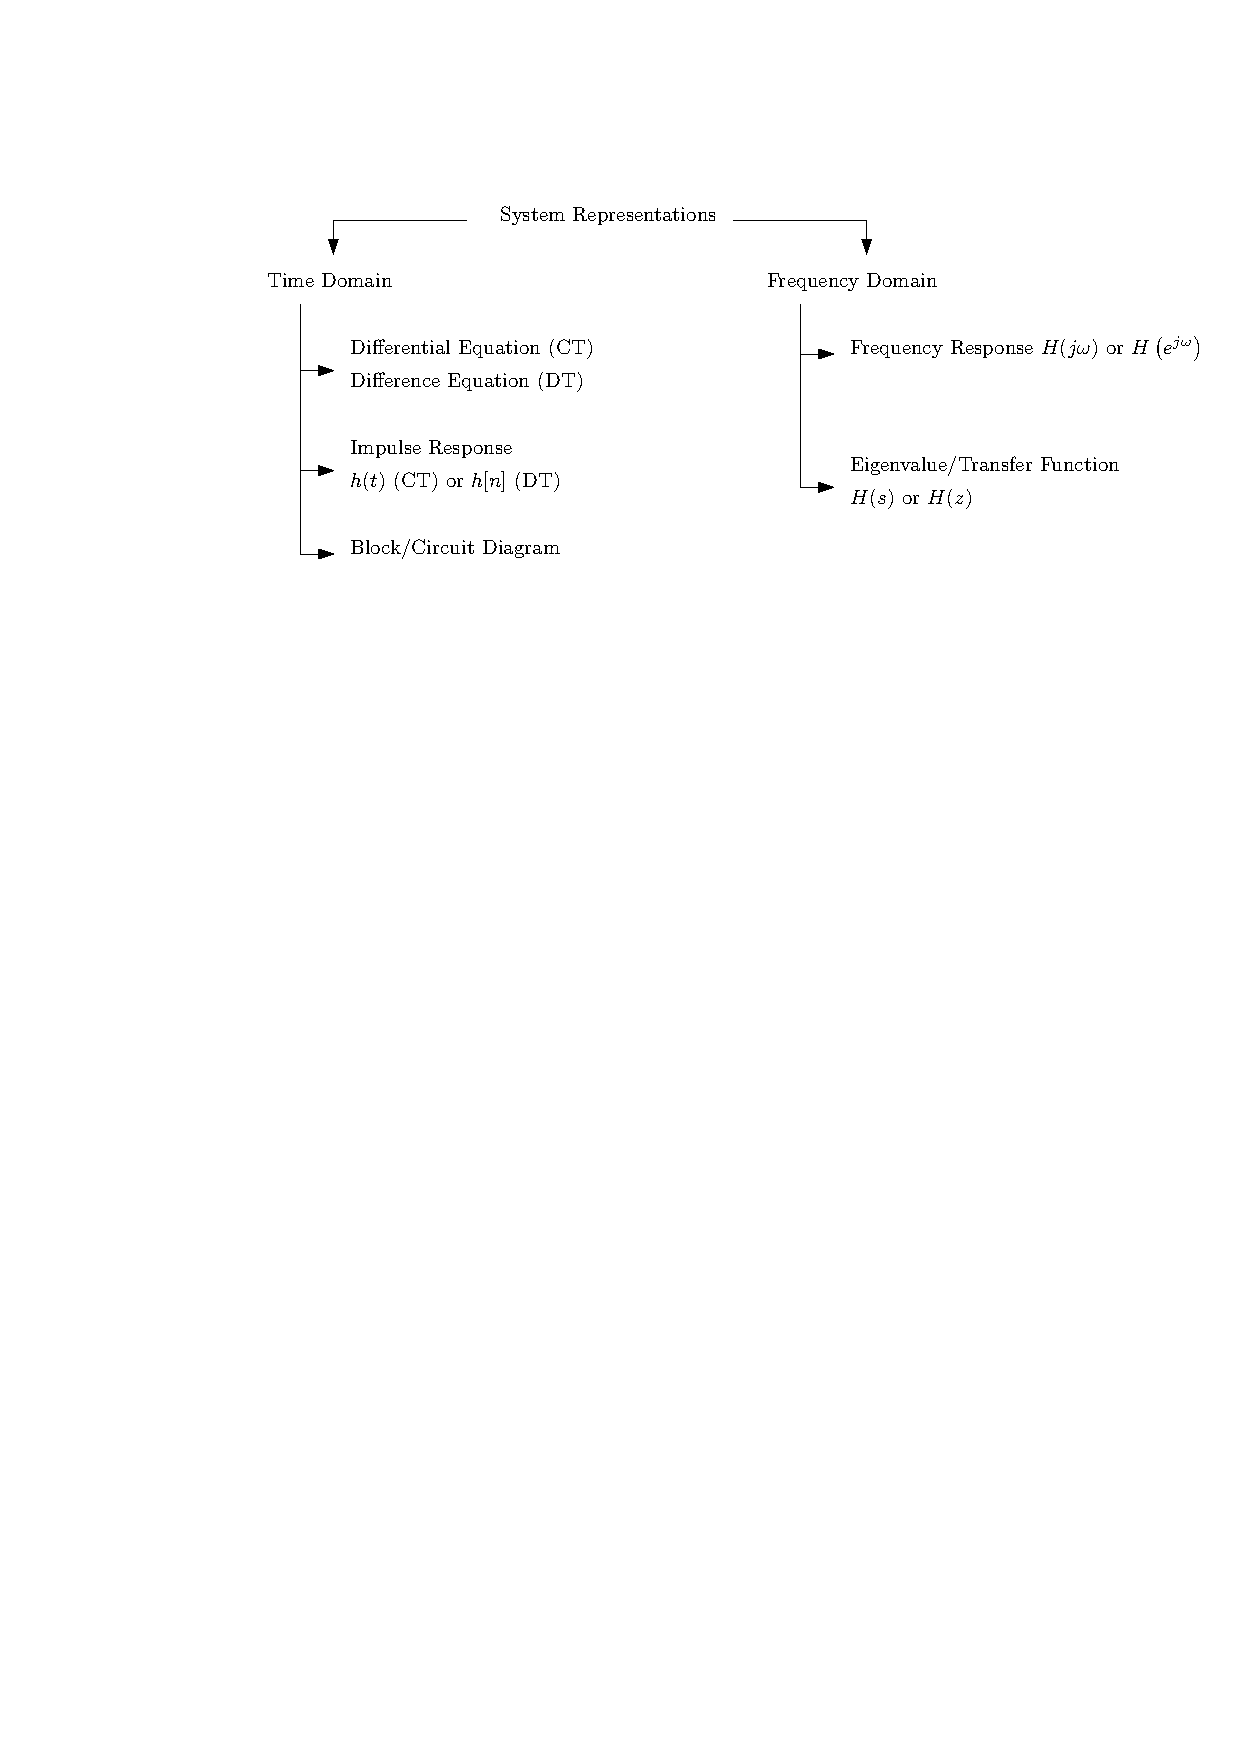
\includegraphics[scale=1]{graphics/system-representations-fig.pdf}
\end{center}
\begin{center}
  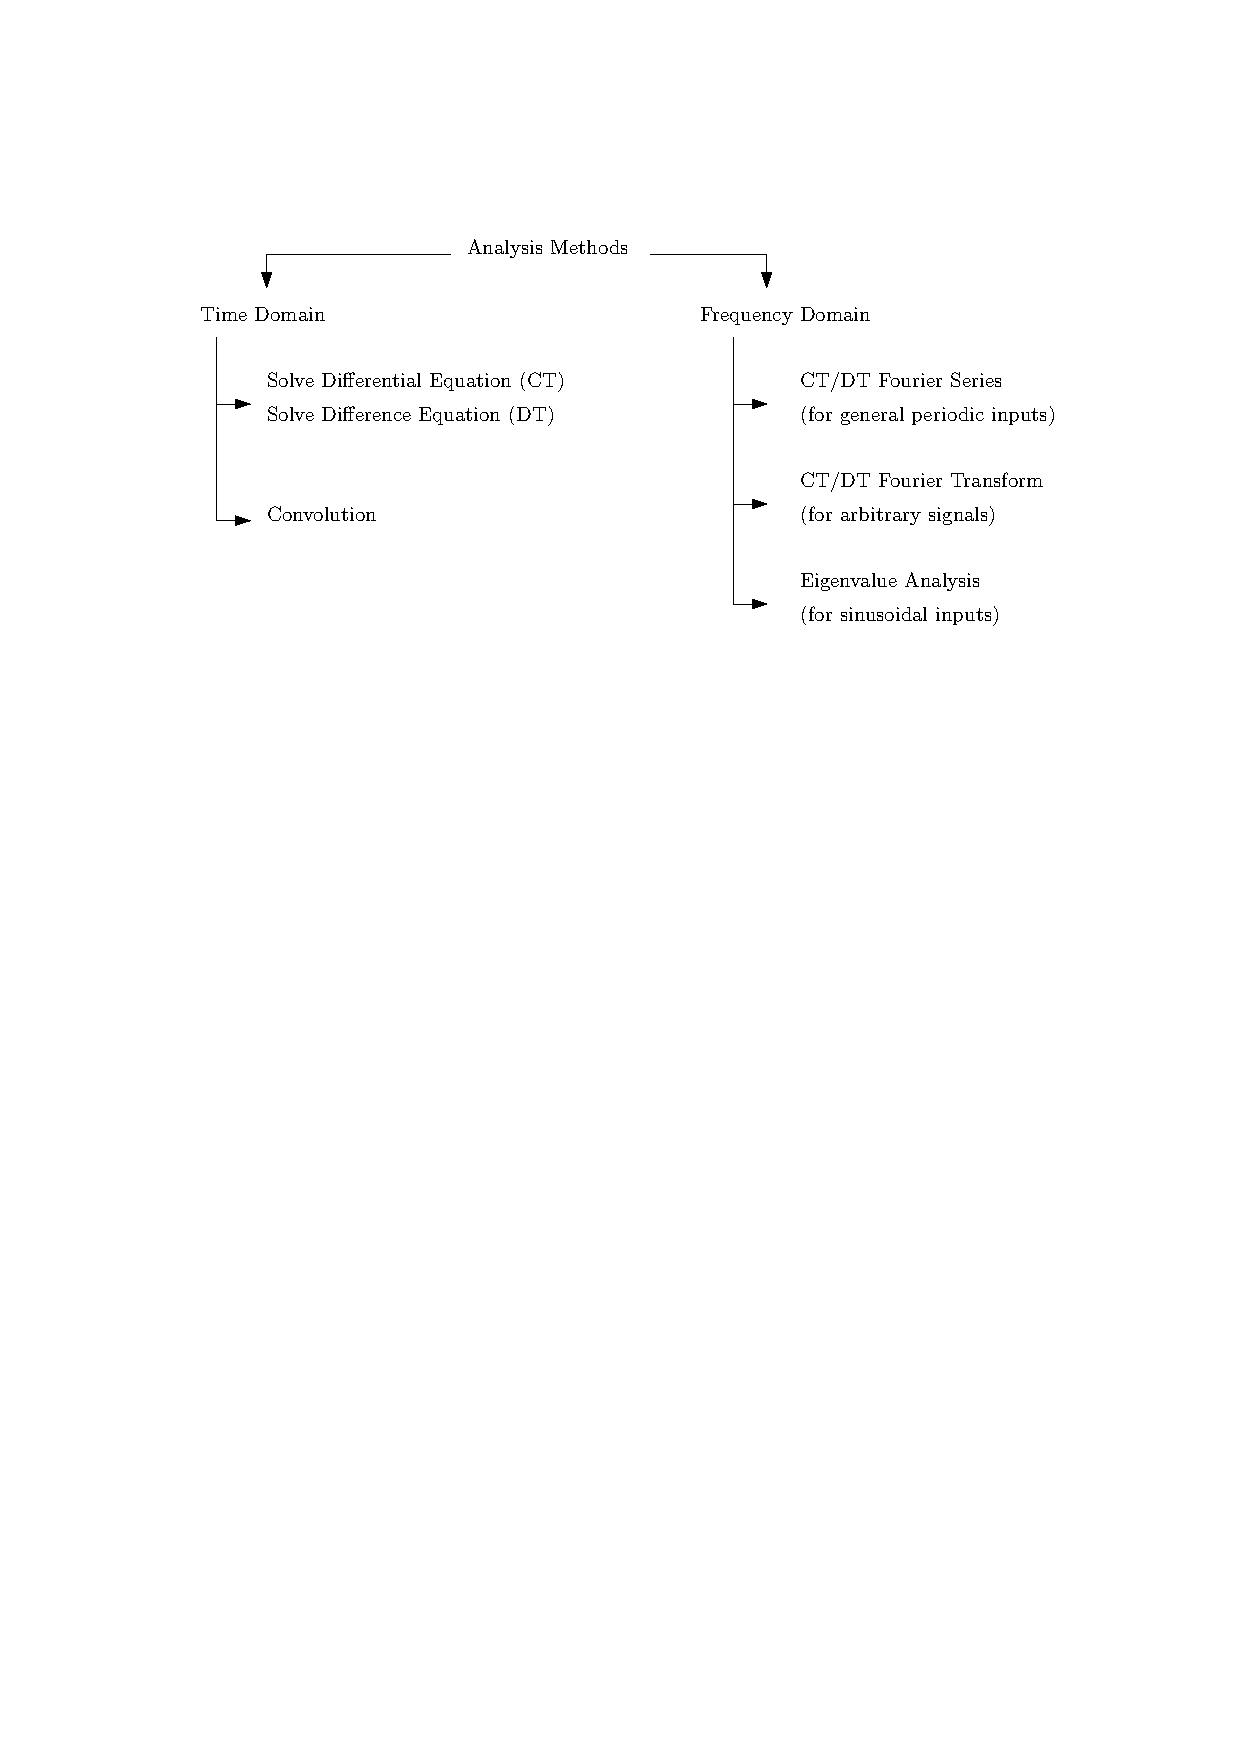
\includegraphics[scale=1]{graphics/analysis-methods-fig.pdf}
\end{center}
